\section{Attività di verifica}
Si analizzano qui le metriche:
\begin{itemize}
    \item \hyperref[s:mpc02]{\textbf{MPC02}}\textbf{}: Budget Variance.
    \item \hyperref[s:mpc04]{\textbf{MPC04}}\textbf{}: Budgeted Cost of Work Scheduled.
    \item \hyperref[s:mpc06]{\textbf{MPC06}}\textbf{}: Actual Cost of Work Performed.
    \item \hyperref[s:mpd1]{\textbf{MPD1}}\textbf{}: Indice di Gulpease.
\end{itemize}

\subsection{MPC02 - Budget Variance}
\label{s:mpc02}
\begin{figure}[htbp]
    \centering
    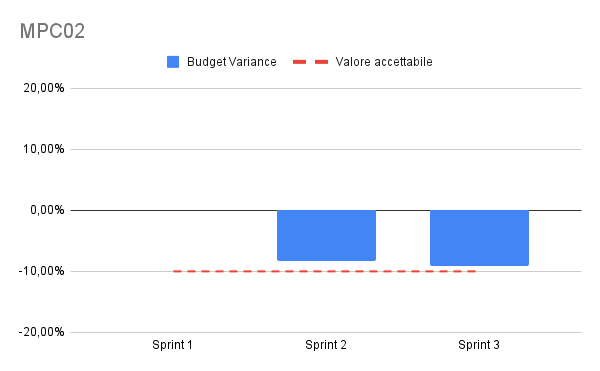
\includegraphics[width=0.7\textwidth]{img/MPC02.png}
    \caption{MPC02 - Budget Variance}
    \label{fig:mpc02}
\end{figure}


\newpage
\subsection{MPC04 - Budgeted Cost of Work Scheduled}
\label{s:mpc04}
\begin{figure}[htbp]
    \centering
    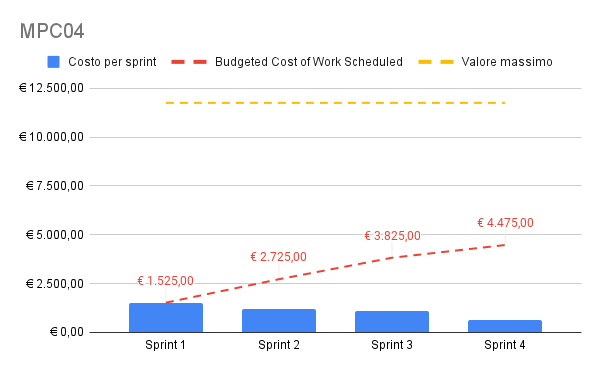
\includegraphics[width=0.7\textwidth]{img/MPC04.png}
    \caption{MPC04 - Budgeted Cost of Work Scheduled}
    \label{fig:mpc04}
\end{figure}

\subsection{MPC06 - Actual Cost of Work Performed}
\label{s:mpc06}
\begin{figure}[htbp]
    \centering
    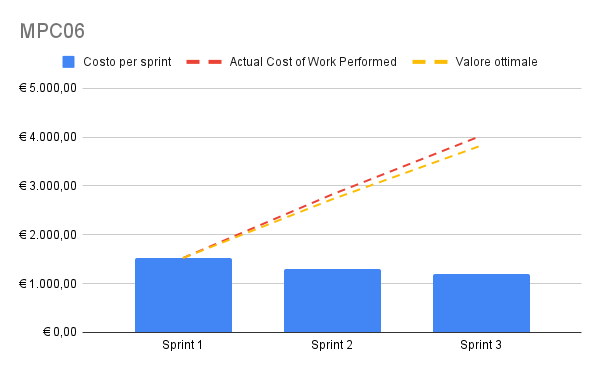
\includegraphics[width=0.7\textwidth]{img/MPC06.png}
    \caption{MPC06 - Actual Cost of Work Performed}
    \label{fig:mpc06}
\end{figure}

\newpage
\subsection{MPD1 - Indice di Gulpease}
\label{s:mpd1}
\begin{figure}[htbp]
    \centering
    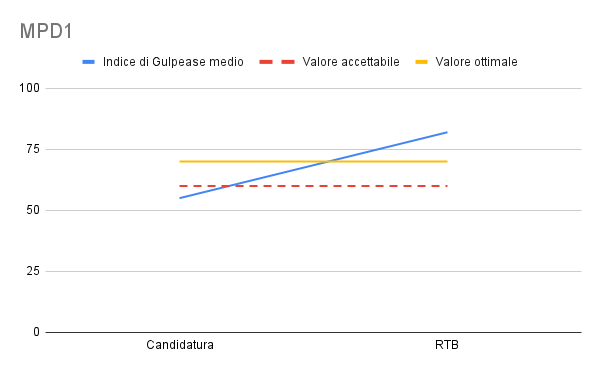
\includegraphics[width=0.7\textwidth]{img/MPD1.png}
    \caption{MPD1 - Indice di Gulpease}
    \label{fig:mpd1}
\end{figure}